\documentclass{article}
\usepackage[utf8]{inputenc}
\usepackage{amssymb}
\usepackage{amsmath}
\usepackage{algorithm2e}
\usepackage{algpseudocode}
\usepackage{graphicx}
\usepackage{cleveref}
\usepackage{geometry}
\usepackage{tikz}
\usepackage{tikz-3dplot}
\usepackage{xcolor}
\usepackage{ifthen}
\usepackage[lambda,
            primitives,
            adversary,
            advantage,
            sets]{cryptocode}

\newcommand{\bb}{\mathbb}
\newcommand{\prgb}{\bb P _\mathsf{RGB}}
\newcommand{\pb}{\bb P _ \mathsf{2}}
\newcommand{\vis}{\approx_v}
\newcommand{\pp}{\bb P}
\newcommand{\pmn}{\pp^{m \times n}}
\newcommand{\hh}{\mathcal H}

\geometry{
 a4paper,
 left=15mm,
 top=20mm,
 right=15mm,
 }
\title{Masters Project - Research}
\author{adrien.laydu}
\date{February 2022}

\begin{document}

\section{Context}

TrustID is an IDP, which stands for a (digital) IDentity Provider that can have various uses, such as 2-Factor Authentication (2FA) or digital signatures. As such, TrustID has to offer ways to securely identify, verify, and authenticate users. To achieve this, TrustID has a strong onboarding procedure, either using a video onboarding process or by having users physically go to an onboarding office, as well as providing an authenticator application for the user's mobile phone. Once onboarded, a user that wants to access a service secured by TrustID enter their credentials ([USERNAME] and password) on the TrustID website. The TrustID server then sends a challenge to the authenticator application, which then uses the unlocking mechanism of the phone to authentify the user: we assume only the targeted user can unlock their phone. The widespread use of biometrics as a way of unlocking phones (rather than traditional passwords or PINs) would ideally improve the security of this method drastically. However, unlocking processes typically offer one of the weaker methods as a fallback. Therefore, TrustID relies only on the ownership of the phone for security.

\vspace{4pt}
That brings us to our security issue: at time of the internship, When the user validates a [TRANSACTION] on their mobile phone (i.e press the ”accept” button of the authenticator app), they have no way of being sure that the prompt on their phone corresponds to the actual [TRANSACTION] they wish to effectuate. This could lead to some vulnerabilities: for example, an impersonation attack is possible, as shown here (we take the example of digital signatures for illustration purposes):

Say an an attacker A wants to sign a document we will call $d_A$ while impersonating user U. U uses a weak password, which means A can log as U on the TrustID website.
\begin{itemize}
    \item A logs as U on TrustID website.
    \item A waits for U to ask for a challenge for any document.
    \item When U asks for a challenge for some document $d_U$, A asks the server for a challenge for $d_A$.
    \item The server will then send two challenges to U’s phone, one for $d_A$ and one for $d_U$.
    \item Since U is unable to distinguish between the two challenges, they validate whichever challenge comes first.
    \item If the challenge for $d_A$ came first, then the attacker successfully signed a document while impersonating U.
\end{itemize}

While not that impactful when used on digital signatures, the same attack could be used for other (much more sensitive) TrustID services, such as 2FA. This project is aimed at solving the security issue presented above. The way we will achieve it is to present the user with a unique, recognizable fingerprint of the document they requested a challenge for. While this could be achieved with traditional hash functions, the fact that human users will have to compare fingerprints calls for a more user-friendly solution. In particular, we want the fingerprints to have the form of pictures, as we hypothesize they are
less cumbersome to compare.

\paragraph{Note:} in practice, A's and U's requests for challenges are augmented with metadata. Different metadata calls for different capabilities of A: a UserID would not call for anything more than assumed earlier. A timestamp (currently in use at time of writing) requires A to send their request simultaneously with U. A nonce would require A to guess the nonce. [MAYBE :] We will see [later] how the choice of metadata alter the probability of a successful attack.

\section{Visual Hashing}

\subsection{Definitions and notations}
\subsubsection{Pixels}
Because we work on image representation, we will work with pixels. We write $\pp$ the set of all pixels. We will often need separate categories of pixels: in particular, we write $\pb \subset \mathbb P$ the set of pixel that may only take two values (namely "white" and "black"). We write $ \prgb \subset \pp$ the set of pixels that are encoded by three color channels (Red, Green, Blue), each channel having an integer value between 0 and 255.
\subsubsection{Visual hash function}
We define a visual hash function as a function $\bin^* \rightarrow \pmn$ of the form: 

$$\hh(x;\lambda) = V(H(x;\lambda);\lambda)$$

Where $\lambda$ is a security parameter, $H : \bin^* \rightarrow \{0,1\}^\ell$ is a standard hash function (such as $\mathsf{SHA-256}$) and $V : \{0,1\}^\ell \rightarrow \mathbb{P}^{m\times n}$ is a mapping from bits strings to arrays of pixels.
The values of $\ell,m,n$ depend on the value of $\lambda$. 

Whenever it is not explicitly needed, we omit the security parameter $\lambda$ in the notation. We call $h := H(x)$ a \textit{hash}, and $F := V(h)$ a \textit{fingerprint}. We note a visual hash function as $\hh = (H,V)$ or when contexts allows it, just $\hh$. 

\subsubsection{Visual indistinguishability}
For two fingerprints $F_1, F_2 \in \pmn$, we write $ F_1 \vis F_2$ if $F_1$ is \textit{visually indistinguishable} from $F_2$, that is, if a user thinks $F_1 = F_2$ by looking at them. Note that $F_1 = F_2 \implies F_1 \vis F_2$. [TO BE CLARIFIED / EXPANDED IN DEDICATED SECTION]
\subsubsection{Properties of visual hash functions}
We adapt traditional hash functions properties to visual hash functions as follows [NOT SURE IF USEFUL YET]. When we say that an attack is "infeasible", we mean that an efficient [DEFINE EFFICIENT - PROBABLY POLY-TIME] adversary cannot realistically perform the attack because of its complexity. The properties are as follows:
\begin{itemize}
    \item \textit{First pre-image resistance}: we say a visual hash function $\mathcal H$ is first pre-image resistant if given $F \in \pmn$, it is infeasible to find $x \in \bin^*$ such that $\mathcal H(x) \vis F$.
    \item \textit{Second pre-image resistance}: we say a visual hash function $\mathcal H$ is second pre-image resistant if given $y \in \bin^*$, it is infeasible to find $x \neq y \in \bin ^*$ such that $\mathcal H(x) \vis \mathcal H(y)$.
    \item \textit{Collision resistance}: we say a visual hash function $\mathcal H$ is collision-resistant if it is infeasible to find $x, y \in \bin ^*$ such that $x \neq y$ and $\mathcal H(x) \vis \mathcal H(y)$.
\end{itemize}
In order to better categorize and analyze visual hash function, we define two additional properties:
\begin{itemize}
    \item \textit{Intermediate pre-image resistance}: we say a visual hash function $\mathcal H = (H, V)$ is intermediate pre-image resistant if given $F \in \pmn$, it is infeasible to find $h \in \bin^\ell$ such that $V(h) \vis F$.
    \item \textit{Visual injectiveness}: we say a visual hash function $\hh = (H,V)$ is visually injective if for any $h_1, h_2 \in \bin^\ell$, $h_1 \neq h_2 \implies V(h_1) \not\vis V(h_2)$. Note that visual injectiveness implies that $V$ is injective, because $V(h_1) \not\vis V(h_2) \implies V(h_1) \neq V(h_2)$
\end{itemize}
\section{Context of application}
\subsection{Protocol}
We consider the protocol shown in \cref{fig:no_adv}, in which a visual hash function $\hh = (H,V)$ is used. On the server side, $\mathsf{md}$ denotes some metadata such as a sessionID, timestamp, nonce, etc. [TO BE EXPANDED IN IMPLEMENTATION SECTION].

\begin{figure}
    \centering
    \procedureblock{\textsc{Verify-Transaction}}{
        \textbf{Server} \< \textbf{Front-end 1} \> \> \textbf{Front-end 2} \> \> \textbf{User} \\
         \> \> \> \> \> \> m \gets \bin^* \\
         \> \sendmessageleftx[9.5cm]{5}{m} \> \\
         t \gets (m || \mathsf{md}) \> \> \> \> \> \> \>  \\
         h \gets H(t) \> \> \> \> \> \> \>  \\
         \> \sendmessageright*[1.5cm]{h} \> \> \> \> \> \> \\[-0.3cm]
        \> \> F_1 \gets V(h) \> \> \> \> \> \> \> \\
        \>  \> \>  \sendmessagerightx{3}{F_1} \> \>   \> \> \\
         \> \sendmessagerightx{3}{h}  \> \\[-0.3cm]
        \> \> \> \> F_2 \gets V(h) \> \> \> \\[-0.5cm]
        \> \>  \> \> \> \sendmessageright*[1.6cm]{F_2} \> \> \> \> \\[-0.3cm]
         \> \> \> \> \> \>F_1 \overset{?}{\approx}_v F_2 \> \\
        }
    \caption{Protocol without adversary.}
    \label{fig:no_adv}
\end{figure}

\subsection{Threat models}
\subsubsection{A realistic TrustID threat}
[GIVE IDEA OF TRANSACTION VALIDATION PROTOCOL (perhaps simplified version of Antoine's UML sequence diagram)]. Following [that], we assume an adversary cannot impersonate the TrustID server. However, an attack by an external adversary is still possible. We define, for an adversary $\adv$, the following game:

\begin{pchstack}[space=2em,center]
    \pseudocode[head = $\mathsf{Game }$ $\Gamma_{\mathsf{TrustID}}$]{%
        m \gets \bin^*\\
        t \gets (m || \mathsf{md})\\
        h \gets H(t)\\
        F \gets V(h)\\
        \adv(t^*) \rightarrow m^\prime\\
        t^\prime \gets (m^\prime || \mathsf{md^\prime})\\
        h^\prime \gets H(t^\prime)\\
        F^\prime \gets V(h^\prime)\\
        \textbf{return }1_{F \vis F^\prime \hspace{3pt} \wedge \hspace{3pt} m^\prime \neq m}
    }
\end{pchstack}
\newcommand{\gid}{\Gamma_{\mathsf{TrustID}}}
Where $t^*$ denotes some part of $t$: depending on the metadata we choose, $\adv$ may know some bits of $t$ that are public (e.g, a timestamp or the user's ID). We consider our scheme achieves the minimal required security if for any efficient adversary $\adv$, $\advantage{\Gamma_{\mathsf{TrustID}}}{\adv}$ is negligible in $\lambda$, where $\advantage{\Gamma_{\mathsf{TrustID}}}{\adv} = \Pr[\Gamma_{\mathsf{TrustID}}$ returns 1]. \Cref{fig:ext_adv} illustrates how the game translates to a concrete implementation.

While we could try and design some visual hash function that achieves this minimal security, we choose to go further and define a stronger threat model: this could alleviate our assumptions on the security of the rest of the TrustID architecture, as well as provide further insight.

\begin{figure}[h]
    \centering
    \procedureblock{\textsc{Verify-Transaction-Realistic}}{%
        \textbf{Adversary} \> \> \textbf{Server} \> \> \textbf{Front-end 1} \> \> \textbf{Front-end 2}  \> \> \textbf{User} \\
        \> \> \> \> \> \> \> \> m \gets \bin^*\\[-0.5cm]
        \> \> \> \sendmessageleftx[9.5cm]{5}{m} \\
        \> \> t \gets (m || \mathsf{md}) \> \> \> \> \> \> \> \\
        \> \> h \gets H(t) \> \> \> \> \> \>  \\[-0.5cm]
        \> \> \> \sendmessageright*[1.5cm]{h} \> \> \> \>\\
        \> \> \> \> F \gets V(h) \> \> \> \> \> \\[-0.5cm]
        \> \> \> \> \>  \sendmessagerightx{3}{F} \> \> \\
        \mathcal{A} \rightarrow m^\prime \> \sendmessageright*[1.5cm]{m^\prime} \> \> \> \> \> \\
        \> \> t^\prime \gets (m^\prime || \mathsf{md}^\prime) \> \> \> \> \>   \\
        \> \> h^\prime \gets H(t^\prime) \> \> \> \> \> \> \\[-0.5cm]
        \> \> \> \sendmessagerightx{3}{h^\prime} \> \\
        \> \> \> \> \> \> F^\prime \gets V(h^\prime) \>\\[-0.5cm]
        \> \> \> \> \> \> \>  \sendmessageright*[1.5cm]{F^\prime} \>\\
        \> \> \> \> \> \> \> \> F \overset{?}{\approx}_v F^\prime \> \\
        }
    \caption{Protocol with a realistic TrustID adversary.}
    \label{fig:ext_adv}
\end{figure}

\newpage

\subsubsection{A stronger threat}

We now define another game, with an adversary $\adv$:
\begin{pchstack}[space=2em,center]
    \pseudocode[head = {$\mathsf{Game}$ $\mathsf{\Gamma}$}]{%
        m \gets \bin^*\\
        t \gets (m || \mathsf{md})\\
        h \gets H(t)\\
        F \gets V(h)\\
        \adv (t,h,F) \rightarrow h^\prime\\
        F^\prime \gets V(h^\prime)\\
        \textbf{return }1_{F \vis F^\prime \hspace{3pt} \wedge \hspace{3pt} h^\prime \neq h}
    }
\end{pchstack}


In words, $\adv$ wins if they can produce a hash $h^\prime$, different from the true hash $h$, that yields a fingerprint $V(h^\prime)$ that is visually indistinguishable from the true fingerprint $F$. 
We will consider our scheme is secure if for any efficient adversary $\adv$, $\advantage{\Gamma}{\adv}$ is negligible in $\lambda$, where $\advantage{\Gamma}{\adv} = \Pr[\Gamma$ returns 1]

We show that this security is indeed stronger that the minimal security we defined in the previous section. Concretely, we prove that, $\advantage{\Gamma}{\adv}$ is negligible for all efficient adversaries $\implies $ $\advantage{\gid}{\adv}$ is negligible for all efficient adversaries. We proceed by reduction: suppose $\adv_\mathsf{TrustID}$ is an efficient adversary playing $\gid$ that wins with non-negligible probability. We build an adversary $\adv$ playing $\Gamma$ that uses $\adv_\mathsf{TrustID}$ to win as follows:

\begin{pchstack}[space=2em,center]
    \pseudocode[head = {$\adv(t,h,F)$}]{%
        \text{Extract $t^*$ from $t$ depending on what $\adv_\mathsf{TrustID}$ needs}\\
        \adv_\mathsf{TrustID}(t^*) \rightarrow m^\prime\\
        t^\prime \gets (m^\prime || \mathsf{md}^\prime)\\
        h^\prime \gets H(t^\prime)\\
        \textbf{return }h^\prime
    }
\end{pchstack}

Note that we suppose that $\adv$ has a way of efficiently knowing $\mathsf{md^\prime}$. Now, if $\adv_\mathsf{TrustID}$ wins at $\gid$, then $\adv$ wins at $\Gamma$. Therefore, $\advantage{\Gamma}{\adv} \geq \advantage{\gid}{\adv_\mathsf{TrustID}}$, which was assumed to be non-negligible, which means $\advantage{\Gamma}{\adv}$ is non-negligible.
That concludes the proof: if there exists an efficient adversary that breaks $\gid$, then there exists an efficient adversary that breaks $\Gamma$. This is equivalent to the statement we wanted to prove.

\Cref{fig:front_adv} illustrate how the threat is stronger: the adversary can bypass the server to submit a hash directly to the frontend.

\begin{figure}[h]
    \centering
    \procedureblock{\textsc{Verify-Transaction-Strong}}{%
        \textbf{Adversary} \> \hspace{1.5cm}\> \textbf{Server} \< \textbf{Front-end 1} \> \hspace{1.5cm} \> \textbf{Front-end 2}  \< \textbf{User} \\[0.5cm]
        \< \< \< \< m\gets \bin^*\\[-0.5cm]
        \< \sendmessageleftx[8.5cm]{10}{m} \> \\
        \< t \gets (m || \mathsf{md}) \< \< \< \\
        \< h \gets H(t) \< \< \< \\[-0.5cm]
        \< \> \sendmessageright*[1.5cm]{h} \> \< \<\\[-0.3cm]
        \< \< F \gets V(h) \< \< \\[-0.3cm]
        \< \< \>  \sendmessagerightx[4cm]{3}{F} \> \\[0.1cm]
        \hspace{0.7cm}\mathcal A \rightarrow h^\prime \< \< \< \< \\[-0.5cm]
        \> \sendmessagerightx[7.5cm]{5}{h^\prime} \< \<  \\[-0.2cm]
        \< \< \< F^\prime \gets V(h^\prime) \< \\[-0.5cm]
        \< \< \< \> \sendmessageright*[1.5cm]{F^\prime} \> \\
        \< \< \< \< F \overset{?}{\approx}_v F^\prime
        }
    \caption{Protocol with a stronger adversary.}
    \label{fig:front_adv}
\end{figure}


\section{Security implications of visual hash function properties}
We separate the different combinations of properties a visual hash function may have, to analyse their strengths and weaknesses in terms of security.
 \subsection{No visual injectiveness, no intermediate pre-image resistance}
\label{section:forge}
If a visual hash function $\hh$ is not intermediate pre-image resistant and isn't visually injective, the adversary can create a forgery:

\begin{enumerate}
    \item From $F$, find $F^\prime \neq F \in \text{Im}(V)$ such that $F \vis F^\prime$.
    \item From $F^\prime$, get $h^\prime$ such that $V(h^\prime) = F^\prime$.
    \item Output $h^\prime$.
\end{enumerate}
This attack is efficient by assumption as long as the adversary can find $F^\prime$ efficiently. Therefore we need at least one of the two proprieties to keep the adversary from making forgeries, or somehow make it infeasible to find $F^\prime$ from $F$.

\subsection{Visual injectiveness}
If $\hh = (H,V)$ is visually injective, then the adversary never wins: indeed, by definition of visual injectiveness, $h \neq h^\prime  \implies V(h) \not\vis V(h^\prime)$. 

Moreover, visual injectiveness implies that the only case where $V(x_1) \vis V(x_2)$ with $x_1 \neq x_2$ is when $H(x_1) = H(x_2)$. That is, in order to find a collision on $\hh$, the adversary must find a collision on $H$. Theferore the following implication holds:
\begin{equation}
    \hh \text{ is visually injective} \wedge H \text{ is collision-resistant} \implies \hh \text{ is collision-resistant}
\end{equation}
\label{eq:sparse}
Since there are well-documented hash functions that are considered collision-resistant, visual injectiveness would be the ultimate goal for our hash function. However we will (probably) see that visual injectiveness is hard to achieve if the input space of $V$ is large (i.e, $\ell$ is large)

\subsection{Intermediate pre-image resistance}
If $\hh = (H,V)$ is intermediate pre-image resistant but isn't visually injective, the attack described in \cref{section:forge} is not feasible, because step 2 is infeasible by intermediate pre-image resistance. [BUT IS IT ENOUGH FOR SECURITY ?]


\section{On visual indistinguishability}
\subsection{Evaluating the difference between fingerprints}
We would like a metric to measure how well our scheme performs, so that we can analyse it formally. In particular, we need to define a distance between $d$ between two fingerprints $F_1,F_2 \in \bb P$ such that for some $\delta > 0$ (ideally as small as possible)
$$d(F_1,F_2) \leq \delta \iff F_1 \vis F_2$$

\subsubsection{normalised Hamming distance}
A natural choice for evaluating the differences between binary images (i.e, that are in $\pb^{m\times n}$) would be to compute the normalised Hamming distance of the two fingerprints
$$d_H(F_1,F_2) = \frac{1}{mn} \sum\limits_{i=0}^{m-1}\sum\limits_{j=0}^{n-1} \mathbb{I}(F_1[i][j] \neq F_2[i][j])$$ where $F_1, F_2 \in \mathbb{P}^{m \times n}$, $(\cdot)[i][j]$ denotes the pixel at position $(i,j)$, and $\mathbb I$ is an indicator function. $d_H$ ranges between 0 and 1 included, the extrema being obtained by having two pictures that differ in zero or all of their pixels, respectively. This metric would be useful because it relates directly to the Hamming distance between of the hashes functions.

Unfortunately, it seems this distance does not achieve the properties we stated above. 
We can refute the right direction ($\implies$) very easily. Indeed, \cref{fig:lowdist} shows two fingerprint with the smallest non-zero Hamming distance ($d_H = \frac{1}{mn}$, $mn = 256$) that are clearly visually distinguishible by humans. Concerning the other direction $(\impliedby)$, we should proceed with caution: shifting bits can produce images that look similar despite having a large Hamming distance. 
\Cref{fig:highdist} shows fingerprints having a normalised Hamming distance of $\frac{71}{256} = 27.73\%$ yet the results are not easy to distinguish.

\begin{figure}[h]
    \centering
    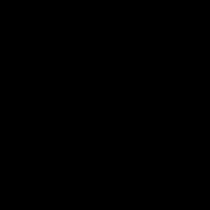
\includegraphics[width=3cm]{figures/0000000000000.png}
    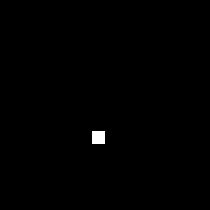
\includegraphics[width=3cm]{figures/0000000001052.png}
    \caption{Two visually distinguishable fingerprints with low Hamming distance.}
    \label{fig:lowdist}
\end{figure}
\begin{center}
\begin{figure}[h]
    \centering
    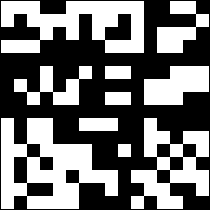
\includegraphics[width=3cm]{figures/e7e6bda110965.png}
    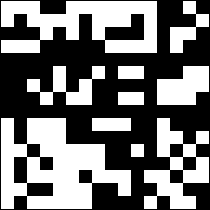
\includegraphics[width=3cm]{figures/e7f2bdd111301.png}
    \caption{Two fingerprints that have a large Hamming distance, but are not trivial to distinguish.}
    \label{fig:highdist}
\end{figure}
\end{center}

\subsubsection{HaarPSI distance}
The Haar perceptual similarity index (HaarPSI) [ref] seems to be a relatively good measure to test whether a pair of fingerprints is distinguishable. The advantages it offers are a relatively low computation time compared to other PSI, which allows for automated parameter search, as well as a good correlation with human opinion scores [ref]. In contrast, the main downside is that although the results are re-linearized, the final output (a number between 0 and 1) is somewhat tricky to interpret: two clearly distinguishable images will have a HaarPSI around 0.1--0.2, and a HaarPSI over 0.6 yields a visual difference that is so small that we consider it imperceptible.

For our future scheme, we would of course like to minimize the HaarPSI distance between any 2 fingerprints. However, given the complexity of the HaarPSI formula, we cannot work our way from that to create a scheme. Instead, we pick a threshold value $T_{Haar} = 0.5$ and we consider that $$\mathsf{HaarPSI}(F_1,F_2) \geq T_{Haar} \implies F_1 \vis F_2$$
The value of $T_{Haar}$ was picked arbitrarily: indeed, determining the value experimentally would require user testing on many subjects, a process for which this project has neither the ambition nor the resources. Note that the condition is necessary but not sufficient: indeed, we empirically found some pairs of fingerprints with a low PSI distance that are not easy to distinguish.


\section{Existing schemes}
\subsection{Antoine's}
Antoine's visual hash is a very simple scheme: $H$ is the standard SHA-256 function, and $V$ is a trivial bit-to-binary pixel mapping (a bit of value 1 gets mapped to a pixel of value 1 (white), a bit of value 0 gets mapped to a pixel of value 0 (black)). It is clear that this scheme is not intermediate pre-image resistant, as the trivial mapping can easily be reversed. Moreover, it is not sparse, as any combination of 256 binary pixels is a valid output: from a fingerprint $F$ one can produce a fingerprint $F^\prime$ that differs from $F$ in only one pixel, which means $F \vis F^\prime$ in general. Therefore, we can conduct the attack described in \cref{section:forge} to create a forgery.
\subsection{LifeHash}
The LifeHash library [ref] employs the standard SHA-256 hash function, but it introduces some complexity in the definition of $b$ using John Conway's Game of Life [ref]. Let $\mathcal{G} : \mathbb P^{m \times n} \rightarrow \mathbb P ^{m \times n}$ be the result of a single generation of the game of life rules on the input. We suppose fingerprints support element-wise addition, as well as multiplication by a constant.

\Cref{algo:lifehash} describes the working of the LifeHash visual hashing function.

\begin{algorithm}
\DontPrintSemicolon
\SetAlgoNoEnd
\KwData{$x \in \bin^*$}
\KwResult{$F \in \prgb^{m_n}$}
\Begin{
    $B \longleftarrow \mathsf{Antoine}(x)$\;  
    Initialize $G$ as the empty array\;
    \While { $|G| < 150$  \textbf{and} Game of Life has not converged}{
        Append $B$ to $G$\; %\Comment{\text{We keep every generation}}
        $B \gets \mathcal{G}(B)$ \Comment{\text{One iteration of Game of Life rules, 1 is alive, 0 is dead}} \;
    }
Initialize $F$ as an all-white (255,255,255) fingerprint the same size as $B$\;
\For {$i = 0, \dotsc, |G|-1$}{
    $F = F - G[i] * \frac{255i}{|G|}$ \Comment{Aggregate all generations}\;
}
Apply RGB mapping to $F$, using some of the first bits to pick a color scheme.\;
Apply symmetry to $F$, using some of the first bits to pick a transformation scheme.\;
\KwRet $F$\;
}
\caption{LifeHash\label{algo:lifehash}}

\end{algorithm}


Due to the unpredictable nature of the Game of Life, one would be tempted to think that this scheme is intermediate pre-image resistant: since one can construct a universal Turing machine in the Game of Life [ref], being able to predict for an arbitrary $h$ the final state of the Game of Life (or even whether the game of life converges in 150 generations) can be reduced to the Halting problem [ref].
But while it may be intermediate resistant on complex inputs, the Game of Life has known, simple patterns that oscillate, which might cause problems if the input hash is simple (i.e. has a low Hamming weight). We describe an example of a forgery in order to illustrate that this scheme is neither intermediate pre-image resistant nor visually injective:

Let the initial state of the Game of Life $B_1$ contain a known oscillator. Let the following state sequence when applying the Game of Life rules successively: $$B_1 \xrightarrow{\mathcal G} B_2 \xrightarrow{\mathcal G}B_3 \xrightarrow{\mathcal G} \dots \xrightarrow{\mathcal{G}} B_1$$

Now, say we have two different input $x_1$ and $x_2$ such that $\mathsf{Antoine}(H(x_1)) = B_1$ and $\mathsf{Antoine}(H(x_2)) = B_2$. Then the execution of \textsc{LifeHash} will go through the same sequence of Game of Life (although rotated one state left for the second), yielding visually similar results. \Cref{fig:lifehash} shows the output picture on input $x_1$ and $x_2$ when 

\begin{align*}
h(x_1) := \hat{h}_1 =\texttt{0000000000000e00e0e0000e00000000eee00000000000006e030002000e0008} \\
h(x_2) := \hat{h}_2 =\texttt{0000000000004e404044404400044440444044400000040064030402000e0008}
\end{align*}

Both hashes contain the same period-3 oscillator (with the same initial state) in the center, and a collection of period-2 oscillators around it: 3 horizontally aligned pixels will flip to 3 vertically aligned pixels back and forth, thus giving a cross pattern on the fingerprint. Both need lcm$(3,2) = 6$ generations of the Game of Life to converge. The fingerprints differ only in the initial direction of the period-2 oscillators: on the left they start horizontally, whereas on the right they start vertically. Because each period-2 oscillators go through 3 entire cycles, the difference between the two setups becomes unnoticeable. 

This pattern is really simple, but it is hard to determine whether other more complicated examples of oscillators combinations yield similar results.


\begin{figure}
    \centering
    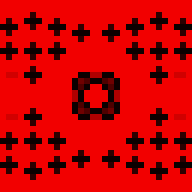
\includegraphics[width=5cm]{figures/ee3.png}
    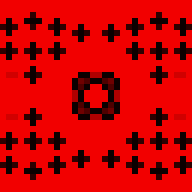
\includegraphics[width=5cm]{figures/443.png}
    \caption{LifeHash outputs when $H = \hat{h}_1$ (left) and $H = \hat{h}_2$ (right)}
    \label{fig:lifehash}
\end{figure}

\subsection{PRG-based libraries}

Some visual hash function use Pseudo-Random Generators (PRG) to create fingerprints. The idea is to seed a PRG with the input value, and let the PRG's randomness act to create fingerprints. Most implementations of such schemes use them directly on the messages (as opposed to hashes), which is not achievable in our case. However, they may have some desirable properties that we analyze in the following sections.

\subsubsection{Blockies}
Blockies [ref] is a light-weight javascript library used to create icons. It is at the time of writing quite popular (more than 1500 weekly downloads according to the official website), following the gain in popularity of cryptocurrency exchange and the need to identify 42-hexadecimal-characters Ethereum addresses.

Blockies is based on a custom-made PRG (!) based on the method used by Java to calculate hashCodes 

\begin{algorithm}
\DontPrintSemicolon
\SetAlgoNoEnd
\KwData{$x \in \bin^*$}
\KwResult{$F \in \prgb^{m \times n}$}
\Begin{
    $\prg_{blockies}.\mathsf{Seed}(x)$ \tcp*[r]{$\prg_{blockies}$ returns values between 0 and 1}\;
    $colorBack  \longleftarrow (\prg_{blockies}.\mathsf{next}()*255,\prg_{blockies}.\mathsf{next}()*255,\prg_{blockies}.\mathsf{next}()*255)$\;
    $colorFront \longleftarrow (\prg_{blockies}.\mathsf{next}()*255,\prg_{blockies}.\mathsf{next}()*255,\prg_{blockies}.\mathsf{next}()*255)$\;
    $colorSpots \longleftarrow (\prg_{blockies}.\mathsf{next}()*255,\prg_{blockies}.\mathsf{next}()*255,\prg_{blockies}.\mathsf{next}()*255)$\;
    \BlankLine\;
    
    Initialize $F$ as an all-zero fingerprint of size $m \times n$
    
    \ForEach{pixel $p$ in $F$ such that $p$ is in the left half of $F$}{
        $val \longleftarrow \prg_{blockies}.\mathsf{next}()*2.3$\;
        \If(\tcp*[f]{happens with prob $\frac{1}{2.3} \approx 43.5\%$}){$val < 1$}{
            $p \longleftarrow colorBack$\;
        }
        \ElseIf(\tcp*[f]{happens with prob $\frac{1}{2.3} \approx 43.5\%$}){$1 \leq val < 2$}{
            $p \longleftarrow colorFront$\;
        }
        \Else(\tcp*[f]{happens with prob $\frac{0.3}{2.3} \approx 13\%$}){
            $p \longleftarrow colorSpots$
            }
    }
    \BlankLine\;
    Set the right half of $F$ to the mirrored left half of $F$
\KwRet $F$\;
}
\caption{PRG-based visual hash function\label{algo:prng}}

\end{algorithm}

\subsubsection{RandomArt}
[Ref] introduces another way of generating visual hashes using randomness: the idea is again to seed a PRG with the hash, then to use recursion to generate a random function to apply to each pixel. To visualise this, we construct an example. We choose a depth of 4, meaning we have 4 level of nesting. The following function was generated : 
\begin{verbatim}
f(x,y) = SUB(SIN(SQRT(DIV(y,0.56))),SIN(ADD(DIV(y,x),SQRT(-0.35))))
\end{verbatim}
In mathematical notation :
$$f(x,y) = \sin{\left(\sqrt{\frac{y}{0.56}}\right)} - \sin\left(\frac{y}{x} + \sqrt{-0.35}\right)$$
Note that each function maps the interval $[-1,1]$ to itself, using the necessary pre-processing if needed, hence the square root of the negative value will not cause any error.

This function is then evaluated at each pixel. \Cref{fig:randomart} shows the resulting fingerprint. In the true scheme, we repeat the process for each color canal.

\begin{figure}
    \centering
    
\includegraphics[width=5cm]{figures/randomart.png}
    \caption{RandomArt visual hash.}
    \label{fig:randomart}
\end{figure}

The issue with this scheme is that the time needed to generate the random function grows exponentially with depth. Also, similarly to the Blockies scheme, the security of RandomHash relies entirely on the security of the PRG. Also, because of the choice of primitives and their properties, different functions can produce the exact same image; for instance 

$$\verb!ADD(MULT(x,y), MULT(0.5, x)) == MULT(x, ADD(y, 0.5))!$$ because $xy + 0.5x = x(y + 0.5)$ for all $x,y$ by distributivity of addition. However, [ref] gives us another tool: the way they evaluated if their hashes were recognisable by humans. Indeed, they give without proof two criteria to assess the quality of their image: 
\begin{itemize}
    \item The fingerprints should have a high compression factor, as low compression is a sign of a chaotic image.
    \item The fingerprints' frequency spectra should be concentrated around low frequences, as high frequences typically indicate noise.
\end{itemize}
The second criterion is what inspired us in the design of our scheme.

\section{Fourier scheme}
The complexity of the RandomHash function generation algorithm grows exponentially with depth, which can incur high computing time. So we design a new scheme with the following idea: instead of generating a random function and hoping that its frequency spectrum is centered around low frequences, we proceed "in reverse" and generate a frequency spectrum centered around low frequences then apply a 2-dimensional inverse Fourier transform to create the image.

\subsection{2D Discrete Fourier Transform}
The 2D Discrete Fourier Transform (2DDFT) is defined as follows:
$$\mathcal{F}(u,v) = \frac{1}{MN}\sum\limits_{x=0}^{M-1}\sum\limits_{y=0}^{N-1}f(x,y) e^{-i2\pi(ux/M + vy/N)}$$
and the 2D Inverse Fourier Transform (2DIDFT):
$$f(x,y) = \sum\limits_{u=0}^{M-1}\sum\limits_{v=0}^{N-1}\mathcal F(u,v) e^{i2\pi(ux/M + vy/N)}$$
where $M$ and $N$ are the dimensions of the input image, and $f(x,y)$ denotes the value of the pixel at position $(x,y)$. Although $\mathcal{F}(u,v)$ is defined for any $u,v \in \mathbb Z$, since $\mathcal F(u + M, v) = \mathcal F(u, v + N) = \mathcal F(u,v)$, we restrict the input domain to $[0,M-1]$ for $u$ and $[0,N-1]$ for $v$ (similarly to how we would sometimes restrict the input domain to $[0, 2\pi)$ for trigonometric functions).

\subsection{Spectrum generation}
What we would like to achieve is to map a hash to an array of coefficients in the frequency domain, and then apply the inverse 2D Transform on this frequency spectrum to get a fingerprint [UNCLEAR]. In this section we give an insight as to how we would generate this spectrum.

First, we have that $\mathcal{F}(u,v)$ is a complex number, meaning each element in the output space of $\mathcal F$ can be thought of as a pair of real numbers (either complex and imaginary parts in a Cartesian system or a modulus and phase in a polar system). 

There is a symmetry in the output space: indeed, we have 
\begin{align*}
    \mathcal{F}(-u,-v) &= \frac{1}{MN}\sum\limits_{x=0}^{M-1}\sum\limits_{y=0}^{N-1}f(x,y) e^{-i2\pi(-ux/M - vy/N)}\\
    &=  \frac{1}{MN}\sum\limits_{x=0}^{M-1}\sum\limits_{y=0}^{N-1}f(x,y) e^{i2\pi(ux/M + vy/N)}\\
    &= \mathcal{F}(u,v)^*
\end{align*}
where $(\cdot)^*$ denotes the complex conjugate. That means we actually have to sample $MN/2$ complex numbers in order to generate a $M \times N$ spectrum.

Figure X shows a graphical representation of how we generate our spectrum. The darker squares represent a number with a greater module.

[SOMETHING ABOUT DISTANCE HERE PROBABLY]

Once the spectrum is generated, the 2DIDFT is applied. The resulting array is then scaled by the inverse of its mean in order to have a mean of 1 [bc very few have values $> 1$], and then multiplied by 255 to get an array of gray pixels. We apply the modulo 255 operator to values greater than 255 to generate the final pixel array. 

\subsubsection{Mapping bits to frequences}
We would like every bit to have roughly the same "importance" with respect to the final image. Therefore, we map words of 4 bits to frequences according to the encoding depicted on figure [FIGURE ENCODING], in which flipping one bit changes both the phase and the module of the resulting frequence. One word is mapped to 2 frequences, which are places according to [FIGURE SPECTRUM].

\Cref{fig:nothing}- shows the resulting fingerprints wits $h = \dots$ and $h^\prime = \dots$. We can see that the results are very hard to distinguish, with a PSI of 0.69 confirming that claim.

\begin{center}
\begin{figure}
    \centering
    
\includegraphics[width=3cm]{figures/Nothing.png}
    \hspace{4pt}
    
\includegraphics[width=3cm]{figures/NothingP67Psi0664}
    \caption{Two fingerprints with one bit flipped}
    \label{fig:nothing}
\end{figure}
\end{center}

\subsubsection{Filtering}

During testing, we noticed that the high-contrast zones due to overflows tend to stand out to the eye and thus help with the distinction of fingerprints [REF WOULD BE NICE]. Therefore, we decided to apply a simple filter to enforce very high contrast zones: namely, from an array $a$ of real values issued from the 2DIDFT, we apply
$$f(a, x,y) = \begin{cases}255 & \text{if }  a(x,y) \geq 0.5\\ 
			0 & \text{otherwise} \end{cases}$$

\begin{center}
\Cref{fig:oneFunc}- shows the two same $h$ and $h^\prime$. As expected, the two images are more easily distinguished (although we will not consider such a small difference to be acceptable). The PSI is 0.242.

\begin{figure}
    \centering
    
\includegraphics[width=3cm]{figures/Filtered.png}
    \hspace{4pt}
    
\includegraphics[width=3cm]{figures/FilteredP67Psi0242.png}
    \caption{The two fingerprints, filtered}
    \label{fig:oneFunc}
\end{figure}
\end{center}

\subsubsection{Number of functions}
\label{rgbSect}

While filtering offers a clear improvement, there is still an issue: we have to map $|h|$ bits to frequences, which results in having to sample spectrum too far away from the axes. To address this problem, we instead perform the sampling procedure [3] times. That way we have 3 spectra array $a_{red}, a_{green}, a_{blue}$, each corresponding to one color channel. The color of a pixel at position is $C(x,y) := (f(a_{red}, x, y), f(a_{green}, x, y), f(a_{blue}, x, y))$ where $f$ is the same filter as in the previous section. \Cref{fig:threeFuncs} shows the two same hashes. We can see that flipping one bit changes one spectrum (in this case, the spectrum corresponding to the blue channel). The resulting images are therefore similarly close to the previous step (Haar-PSI = 0.23).

\begin{center}
\begin{figure}
    \centering
    
\includegraphics[width=3cm]{figures/ThreeFuncs.png}
    
\includegraphics[width=3cm]{figures/ThreeFuncsP67Psi0232.png}
    \caption{The two fingerprints, with 3 functions}
    \label{fig:threeFuncs}
\end{figure}
\end{center}

\subsubsection{Colors}

As we have just seen, a difference in colors helps with distingishibility. We would thus have a lot to gain picking a different set of colors for different hashes. As we would like to use colors more colors than the combinations of the pure colors (colors that have only one non-zero), we must slightly change the way we assign a color to a pixel: we must choose $2^3$ colors to account for every possibility of the filtered values of $a_0, a_1$ and $a_2$. Suppose we have an array named $Colors$ of length 8, containing rgb encodings.
\begin{table}
	\begin{center}
	\begin{tabular}{c|c}
		Filtered values of $a_0(x,y)$, $a_1(x,y)$, $a_2(x,y)$ & $C(x,y)$\\
		\hline 0,   0,   0 & $Colors[0]$\\
		 0,   0, 255 & $Colors[1]$\\
		 0, 255,   0 & $Colors[2]$\\
		 0, 255, 255 & $Colors[3]$\\
		 255,   0,   0 & $Colors[4]$\\
		 255,   0, 255 & $Colors[5]$\\
		 255, 255,   0 & $Colors[6]$\\
		255, 255, 255 & $Colors[7]$\\
	\end{tabular}
	\caption{Color mapping}
	\end{center}
\end{table}

Note that the system described in \cref{rgbSect} corresponds to picking the color to be the filtered values directly. To choose the set of 8 colors that will make the output set of $C(x,y)$, we use parity bits:

Let the parity bits $p_0$ to $p_{15}$ be defined as 
\begin{equation*}
	p_i = \begin{cases} 
	    b_{i} \oplus b_{12+i} \oplus b_{24+i} \oplus \dots \oplus b_{108+i} = \bigoplus_{k=0}^9 b_{12k+i} & 0 \leq i < 12\\
	    b_{108 + i} \oplus b_{112 + i} & 12 \leq i < 16
	    \end{cases}
\end{equation*}

We compute the colors indices:
 $$c_j = p_{2j} || p_{2j+1} \text{ for } j \in \{0,\dotsc,7\}$$ where $||$ denotes concatenation, therefore $c_j \in \{0,1,2,3\}$.
 Let $Palette$ be a fixed 32 colors palette. We fill $Colors$ as :
$$Colors[j] = Palette[4j + c_j] \text{ for } j \in \{0, \dotsc, 7\}$$
Figure [FIGURE] depicts this process, and \cref{fig:threeFuncsColor} shows the two hashes. We can see that flipping one bit results in one color change. While in our case the results are quite obviously different (Haar PSI = 0.25 [COMMENT ON THIS]), there are cases where only a very small portion of the image is of a certain color, which would yield almost no difference should this color be changed.

\begin{center}
\begin{figure}
    \centering
    
\includegraphics[width=3cm]{figures/Colors.png}
    
\includegraphics[width=3cm]{figures/ColorsP67Psi0255.png}
    \caption{The two fingerprints, with 3 functions}
    \label{fig:threeFuncsColor}
\end{figure}
\end{center}

An even stronger attack would be to flip 2 bits that correspond to the same parity bit: flipping both $b_j$ and $b_{j+12k}$ yields a fingerprint that differs only in the shapes of the patterns, which may not be significant enough.

\subsubsection{Palette shifting and reversing}
As having only one color changed may result in very little zones switching colors, we would like to change more than one color if one bit is flipped. To achieve that, we apply a transformation to the palette before extracting the colors: namely, we shift it by $h \mod p$, where $h$ is interpreted as a 128-bit integer, and $p$ is a prime number less than 32 [MAYBE JUST ODD NUMBER] to be determined later. In addition, if the Hamming weight of the hash is odd, that is, if $\sum\limits_i b_i \mod 2 = 1$, we reverse the palette. That way, flipping an odd number of bits is guaranteed to have almost every color changed [PROOF?]. There are still possible collisions though: due to the fact that we have to pick a small prime, there exists some $h^\prime$ that differ from $h$ at an even number of indices that use the same palette and colors as $h$. For example, if we were to flip two bits at indices $\ell$ and $k$,  we would have the same palette shift if 
$h^\prime = h + 2^\ell - 2^k = h \mod p$ and the bits at indices $k$ and $\ell$ are different, or if $h^\prime + 2^\ell + 2^k = h \mod p$ and the bits at indices $k$ and $\ell$ are equal. The scenario we want to avoid is two have both $h$ and $h^\prime$ use the exact same colors, that is, have the same palette shift and the same parity bits.
This happens if 

$$	h + \sum\limits_\ell 2^\ell - \sum\limits_k 2^k = h \mod p $$

If only two bits are changed we have
\begin{align*}
	h + 2^k - 2^{k+12m} &= h \mod p\\
	h + 2^k(2^{12m} - 1) &= h \mod p \\
	2^k (2^{12m} - 1) &= 0 \mod p \\
	2^{12m} - 1 &= 0 \mod p \\
	2^{12m} &= 1 \mod p \\
	12m &= 0 \mod (|2| \mod p)
\end{align*}

This constraint helps with the choice of $p$: indeed, we would like to maximize lcm$(12, |2| \mod p)$ so that we minimize the number of pairs that satisfy the constraint. In particular, good candidates are $p= 23$ (lcm$(12, |2| \mod p) = 132$) and $p=29$ (lcm$(12, |2| \mod p) = 84$)

\subsubsection{Symmetries}
While changing colors is a great way to achieve significant visual differences, there humans tend to perform better at identifying symmetrical objects [ref]. Therefore, we would like our fingerprints to be symmetric. The way we do this is to first generate the fingerprint as we did previously, and then apply some symmetry according to a symmetry mode [DETAILS].

In order to determine the symmetry mode, we simply compute $h \mod q$, where $q \neq p$ is a small prime (in the order of 20). 

To have the same the same symmetry, one would have to achieve $k - \ell = 0\mod (|2| \mod q)$. Having the same palette shift AND same symmetry yields
$$\begin{cases}
k - \ell &= 0 \mod (|2| \mod p)\\
k - \ell &= 0 \mod (|2| \mod q)
\end{cases} \iff k - \ell = 0 \mod \text{lcm}(|2| \mod p, |2| \mod q)$$.

Picking $p, q \in \{23, 29\}$ yields $\text{lcm}(|2| \mod p, |2| \mod q) = \text{lcm}(11, 28) = 308$. Therefore, if 2 bits are flipped, then either the palette is shifted differently, or the symmetry is not the same, or both. Either of these cases yields visually distinguishable results.

\subsection{Worst cases}
We now analyse the worst case scenarios against our scheme. Let us assume $n$ bits were flipped. Let us pick $p=29, q=23$. We have $pq = 667$, $|2| \mod p = 28, |q| \mod q = 11$
\begin{itemize}
	\item $n=1$ : The palette is flipped, the shift is different, the symmetry is different.
	\item $n=2$ : Either the shift is different, the symmetry is different, or both.
	\item $n > 2, n$ odd : The palette is flipped.
\end{itemize}
For an even $n > 2$, there are collisions in the sense that some pairs of hashes use the same palette, same colors and same symmetry.
\begin{itemize}
	\item For $n = 4$, we have $2^0 + 2^{84} + 2^{96} + 2^{108} \equiv 0 \mod 667$ which means flipping bits with indices $0 + d, 84 + d, 96 + d, 108 + d$ with $d \in \{0 \dots 11\}$ yields the same configuration if all the bits at these indices have the same value. We estimate the probability that $h$ contains a 4 bits of same value at at least one of the possibilities for $d$ to be $\left(1 - \frac{1}{8}\right)^{12} = \left(\frac{7}{8}\right)^{12} \approx \frac{1}{5}$. (Note that this estimation assumes independent and uniform bits, which is not guaranteed but we just want to show that the probability is very big). Because that is a very high probability, we need patterns to change enough when 4 frequences are changed. Empirically, this seems to be the case
\end{itemize}

\subsection{Randomness}
While having a scheme relying entirely on a PRG is not desirable [WHY?], we may use randomness when generating the $\omega_i$ in order to achieve intermediate pre-image resistance. In particular, we tried randomizing any combination of the $\omega_i$ moduli and phases. \Cref{tab:detvsrand} shows the computation of the $\omega_i$, where $d_i$ is the evaluation of a distance function at the coordinates of the pixel corresponding to $b_i$. The exact formula for $d_i$ is described [LATER].

\begin{table}[]
    \centering
    \begin{tabular}{|c|c|c|}
    \hline
        & Deterministic Phase & Random Phase \\
        \hline
        Deterministic module    & $\omega_i = d_i \cdot (0.5 + 0.5b_i) /// 1 \cdot \exp{(b_i \cdot \pi i)}$ & $\omega_i = d_i \cdot b_i\exp{(rand() \cdot 2 \pi i )}$\\
        \hline
        Random module & $\omega_i = d_i \cdot rand() \cdot \exp{(b_i \cdot \pi i)}$ & $\omega_i = d_i \cdot rand()\cdot \exp{(rand() \cdot 2\pi i)}$\\
        \hline
    \end{tabular}
    \caption{Caption}
    \label{tab:detvsrand}
\end{table}

\subsection{Distance function}
We want our $\omega_i$ to have high modules around the axes. That being said, we have to decide exactly which function must the modules follow. We tried several options, detailed in \cref{tab:distances}.

\subsection{(Temporary) Fourier visual hash scheme}


\begin{table}[]
    \centering
    \def\arraystretch{1.5}
    \begin{tabular}{|c|c|}
        \hline
        Name & Formula \\
        \hline
        \verb!MANHATTAN! &  $\frac{1}{|x| + |y|}$\\
        \verb!SQUARE! &  $\frac{1}{x^2 + y^2}$\\
        \verb!CUBIC! &  $\frac{1}{|x|^3 + |y|^3}$\\
        \verb!EUCLIDEAN! &   $\frac{1}{\sqrt{x^2 + y^2}}$\\
        \verb!CUBIC! & $\frac{1}{x^3 + y^3}$\\
        \verb!MULT! &  $\frac{1}{|xy|}$\\
        \verb!XY! &  $\frac{|xy|}{x^2 + y^2}$\\
        \verb!BELL! & $e^{-(x^2 + y^2)/3}$\\
        \verb!SIGMOID! & if $\frac{1 - 2\max(|x|,|y|)}{(1-2t)(1 + e^{-0.01|xy|})}$\\
        \hline
    \end{tabular}
    \caption{Caption}
    \label{tab:distances}
\end{table}


\end{document}

\subsection{First pre-image resistance}
We claim that 
\begin{equation}
    H \text{ is first pre-image resistant} \implies \hh \text{ is first pre-image resistant}
\end{equation}
\label{eq:firstpre}
The proof is as follows: an adversary that is given $\hh(x) = V(H(x))$ may recover information about $H(x)$. From there, to recover $x$, the adversary must find a pre-image on $H$. Therefore, by contraposition, an adversary able to conduct a pre-image attack on $\hh$ must be able to conduct a pre-image attack on $H$, which means the implication holds.

This implication is greatly useful because there are well-documented hash functions that are considered first pre-image resistant [ref]. Therefore, by choosing one such hash function for $H$, we can achieve first pre-image resistance on $\hh$ regardless of the properties of $V$.

We assume an adversary may have any combination of the following capabilities:
\begin{itemize}
    \item Know some part of $t$ (e.g $m$ or the metadata).
    \item Know $t$
    \item Know $F$.
    \item Know $h$.
\end{itemize}

\subsubsection{Adversary types}
\paragraph{Front-end adversary}
\Cref{fig:frontend-adv} illustrates the strongest type of adversary, which we call a front-end adversary as the adversary impersonates one of the front-ends. A front-end adversary is unrealistic in practice: having access to the front-end would mean hacking the user's browser and modify the source code, which we consider infeasible. Therefore, we will not consider front-end adversaries in our analysis.
\paragraph{Back-end adversary}
\Cref{fig:backend_adv} shows the second strongest type of adversary, which we call a back-end adversary. A back-end adversary may for example be a man-in-the-middle between the server and one of the front-ends, that is able to force one of the front-ends to display a fingerprint corresponding to a chosen bit string. 
\paragraph{External adversary}
\Cref{fig:backend_adv} shows the weakest type of adversary, which we call an external adversary. An external adversary may be a malicious user that tries to make the user validate $m^\prime$  instead of $m$.
\subsubsection{Considered threat model}
In our analysis, we consider the most powerful realistic adversary, that is, a back-end adversary that knows $t, h$ and $F$. Formally, we define for any efficient [DEFINE EFFICIENT - POLYTIME ?] adversary $\adv$ the following game:

V strongly sparsed + H collision-resistant => \hh collision-resistant








\begin{figure}
    \centering
    \procedureblock{\textsc{Verify-Transaction-FrontEnd-Adv}}{%
        \textbf{Adversary} \> \hspace{1.5cm}\> \textbf{Server} \< \textbf{Front-end 1} \> \hspace{1.5cm} \> \textbf{Front-end 2}  \< \textbf{User} \\[0.5cm]
        \< \< \< \< m\gets \bin^*\\[-0.5cm]
        \< \sendmessageleftx[8cm]{10}{m} \> \\[-0.3cm]
        \< t \gets (m || \mathsf{md}) \< \< \< \\
        \< h \gets H(t) \< \< \< \\[-0.5cm]
        \< \> \sendmessageright*[1.5cm]{h} \> \< \<\\[-0.3cm]
        \< \< F \gets V(h) \< \< \\[-0.3cm]
        \< \< \>  \sendmessagerightx[4.5cm]{3}{F} \> \\
        \hspace{0.7cm}\mathcal A \rightarrow F^\prime \< \< \< \< \\[-0.5cm]
        \> \sendmessagerightx[12cm]{7}{F^\prime} \< \<  \\
        \< \< \< \< F \overset{?}{\approx}_v F^\prime
        }
    \caption{Protocol with front-end adversary.}
    \label{fig:back-end_adv}
\end{figure}
\begin{figure}
    \centering
    \procedureblock{\textsc{Verify-Transaction-Strong}}{%
        \textbf{Adversary} \> \hspace{1.5cm}\> \textbf{Server} \< \textbf{Front-end 1} \> \hspace{1.5cm} \> \textbf{Front-end 2}  \< \textbf{User} \\[0.5cm]
        \< \< \< \< m\gets \bin^*\\[-0.5cm]
        \< \sendmessageleftx[8.5cm]{10}{m} \> \\
        \< t \gets (m || \mathsf{md}) \< \< \< \\
        \< h \gets H(t) \< \< \< \\[-0.5cm]
        \< \> \sendmessageright*[1.5cm]{h} \> \< \<\\[-0.3cm]
        \< \< F \gets V(h) \< \< \\[-0.3cm]
        \< \< \>  \sendmessagerightx[4cm]{3}{F} \> \\[0.1cm]
        \hspace{0.7cm}\mathcal A \rightarrow h^\prime \< \< \< \< \\[-0.5cm]
        \> \sendmessagerightx[7.5cm]{5}{h^\prime} \< \<  \\[-0.2cm]
        \< \< \< F^\prime \gets V(h^\prime) \< \\[-0.5cm]
        \< \< \< \> \sendmessageright*[1.5cm]{F^\prime} \> \\
        \< \< \< \< F \overset{?}{\approx}_v F^\prime
        }
    \caption{Protocol with a stronger adversary.}
    \label{fig:front_adv}
\end{figure}

\begin{figure}
    \centering
    \procedureblock{\textsc{Verify-Transaction-External-Adv}}{%
        \textbf{Adversary} \> \> \textbf{Server} \> \> \textbf{Front-end 1} \> \> \textbf{Front-end 2}  \> \> \textbf{User} \\
        \> \> \> \> \> \> \> \> m \gets \bin^*\\
        \> \> \> \sendmessageleftx[9.5cm]{5}{m} \\
        \> \> t \gets (m || \mathsf{md}) \> \> \> \> \> \> \> \\
        \> \> h \gets H(t) \> \> \> \> \> \>  \\[-0.5cm]
        \> \> \> \sendmessageright*[1.5cm]{h} \> \> \> \>\\
        \> \> \> \> F \gets V(h) \> \> \> \> \> \\[-0.5cm]
        \> \> \> \> \>  \sendmessagerightx{3}{F} \> \> \\
        \mathcal{A} \rightarrow m^\prime \> \sendmessageright*[1.5cm]{m^\prime} \> \> \> \> \> \\
        \> \> t^\prime \gets (m^\prime || \mathsf{md}^\prime) \> \> \> \> \>   \\
        \> \> h^\prime \gets H(t^\prime) \> \> \> \> \> \> \\[-0.5cm]
        \> \> \> \sendmessagerightx{3}{h^\prime} \> \\
        \> \> \> \> \> \> F^\prime \gets V(h^\prime) \>\\[-0.5cm]
        \> \> \> \> \> \> \>  \sendmessageright*[1.5cm]{F^\prime} \>\\
        \> \> \> \> \> \> \> \> F \overset{?}{\approx}_v F^\prime \> \\
        }
    \caption{Protocol with external adversary.}
    \label{fig:ext_adv}
\end{figure}

\subsubsection{Hamming distance for color pixels}
It is clear that for color pixels, i.e if $F_1, F_2 \in \prgb^{m \times n}$, the Hamming distance is a terrible metric, since every pixel from $F_1$ differ from their counterpart in $F_2$ in only one channel, by a small value (1) then the Hamming distance is $m \times n$ (maximal), but the two pictures will look almost the same since it is hard/very hard/impossible for humans to distinguish between colors that are so close to eath other [ref] 
%%%%%%%TODO : FIND REF%%%%%%%%%%%%%%%

\begin{figure}
    \centering
    
\includegraphics[width=3cm]{figures/20254100.png}
    
\includegraphics[width=3cm]{figures/20255100.png}
    \caption{Visually close fingerprints with maximal hamming distance (L: (20,254,100), R: (20,255,100))}
    \label{fig:closecolors}
\end{figure}

For that reason we introduce the RGB-Hamming distance:

$$d_H^\mathsf{RGB} (F_1,F_2)= \frac{1}{256^3mn}\sum\limits_{i=0}^{m-1}\sum\limits_{j=0}^{n-1}\sum_{c = \{R,G,B\}}(F_1[i][j])_c - (F_2[i][j])_c$$
where $F_1,F_2 \in \prgb ^{m\times n}$ and $(F_x[i][j])_c \in \{0, \dotsc ,255\}$ denotes the value of the color channel corresponding to $c$ of the pixel at position $(i,j)$ of $F_x$




\Cref{fig:unfiltered} shows the resulting fingerprints of [$h$ and $h^\prime$], that differ only at bit 67. This pair yields a Haar-PSI value of 0.883, which is much more than the threshold value [OF X]

\begin{center}
\begin{figure}[h]
    \centering
    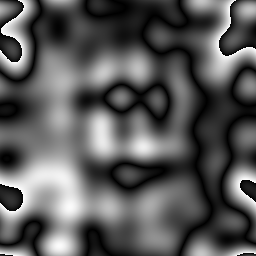
\includegraphics[width=3cm]{figures/OneFunc_Unfiltered.png}
    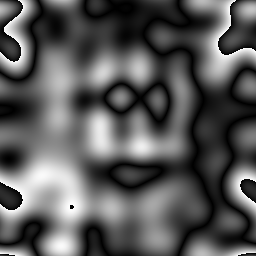
\includegraphics[width=3cm]{figures/OneFuncP67_Unfiltered.png}
    \caption{Two fingerprints that differ only in one bit}
    \label{fig:unfiltered}
\end{figure}
\end{center}